\chapter{Imaging the Extended Groth Strip with the full LOFAR array}
\minitoc
\section{Aims \& Methodology}

\pg
primary aim: see if direction-independent calibration of EGS good enough, for international baselines, to allow for HR imaging of entire EGS with acceptable upper bounds to decorrelation throughout field.
\pg
in other words: can entire EGS be placed on same facet as 3C295 at high resolutions? Link to V.

\pg
necessary test: investigate impact of decorrelation as function of distance from 3C295 (calibrator) - do we lose enough signal to lose resolution?

\pg LOBOS survey gives list of VLBI phase calibrators in primary beam: compact sources, should show impact of direction-dependent gain errors directly. These are distributed at various distances from 3C295, conveniently.
\pg
Show images (+ overlays?) of direction-dependent PSF (i.e. modelled decorrelation due to time-freq averaging) and images of LOBOS sources

\pg
Finally, show plot of ratio of $flux_{peak}$ / $flux_{integrated}$ as function of distance from 3C295: the flatter, the better.

\pg
Imaging strategy: image the field patch by patch.
\pg
Have source list of entire EGS from section V. Use that to subtract all source save those in the patch from visibilities, then image (self-cal?) over that patch. Rinse and repeat throughout EGS.


\section{Testing Decorrelation - LOBOS Sources in the Primary Beam}

\pg
describe LOBOS catalogue \& sources chosen  - why, how

\begin{table}[h!]
\begin{tabular}{ccccc}
\# & RA [hms]    & Dec [dms]   & Dist. from EGS [deg.] & Dist. from 3C295 [deg.] \\\hline
1  & 14:30:18.72 & 52:17:29.80 & 2.041                         & 2.904 \\
2  & 14:19:44.44 & 54:23:04.58 & 1.928                         & 2.517 \\ 
3  & 14:21:20.05 & 53:03:46.00 & 0.864                         & 1.743 \\
4  & 14:21:09.41 & 51:22:32.46 & 1.294                         & 1.728 \\
5  & 14:11:50.32 & 52:49:02.66 & 0.844                         & 0.619 \\
6  & 14:11:20.23 & 52:12:04.30 & 0.915                         & 0.000 \\
7  & 14:08:07.00 & 52:55:11.36 & 1.409                         & 0.869 \\
8  & 14:08:09.76 & 52:44:46.56 & 1.354                         & 0.680 \\
\end{tabular}
\caption{\label{table.LOBOS.sources}Table recapitulating the positions of all 8 chosen calibrator sources, along with their distance from the observation phase centre (EGS phase centre) and calibrator phase centre (3C295), respectively.}
\end{table}
\begin{figure}[h!]
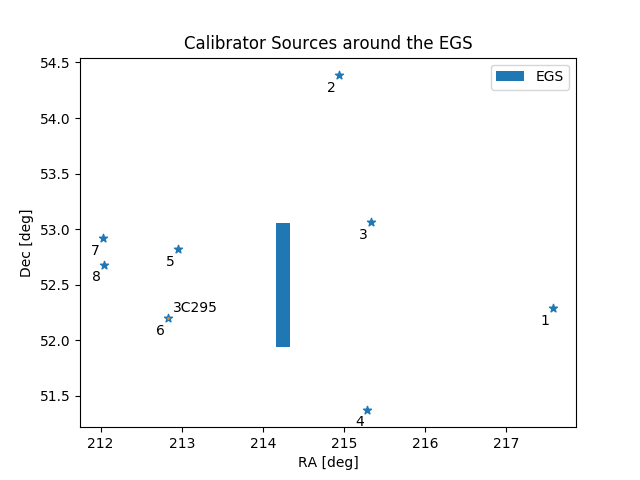
\includegraphics[width=0.8\linewidth]{images/EGS_LOBOS_scatterplot}
\caption{Position of the calibrator sources around the EGS. Note that this is not projected properly onto the celestial sphere.}
\label{bootes-coverage-image}
\end{figure}

\pg
show images of decorrelation, residuals etc for all 8 sources


\section{Patchwise Imaging of the EGS using LOFAR International Stations}

\newpage